\documentclass{beamer}
\usetheme{AnnArbor}
\usecolortheme{beaver}
\usepackage{amsmath}
\usepackage{ragged2e}
\justifying 

\title[Implementation of the PLS algorithm]{Implementation in MATLAB of the Partial Least Squares algorithm for classification}
\subtitle{Case study: fault detection and diagnosis on steel plates}
\author[L. Ferrari, L. Leoni]{Lorenzo Ferrari \and Lorenzo Leoni}
\institute[University of Bergamo]{ Department of Engineering and Applied Sciences, University of Bergamo}
\date{\today}

\begin{document}
	
	\begin{frame}
		\titlepage
	\end{frame}

	\begin{frame}
		\frametitle{Outline}
		\tableofcontents
	\end{frame}
	
	\section{Introduction}

\begin{frame}
	TO DO
\end{frame}
	\section{Description of the PLS  algorithm}

\begin{frame}[fragile]
	\frametitle{NIPALS algorithm}
	The most popular algorithm used in PLS to compute the model parameters is known as \textbf{non-iterative partial least squares} (\textbf{NIPALS}). There are two versions of this technique:
	\begin{itemize}
		\item \textbf{PLS1}: each of the \textit{p} predicted variables is modeled separately, resulting in one model for each class;
		\item \textbf{PLS2}: all predicted variables are modeled simultaneously.
	\end{itemize}
	The first algorithm is more accurate than the other, however it requires more computational time than PLS2 to find the $\alpha$ eigenvectors into which project the \textit{m} covariates. 
\end{frame}

\begin{frame}
	\frametitle{Data structures}
	Before starting with the description of the algorithm, we recall that:
	\begin{itemize}
		\item the matrix $X \in \mathbb{R}^{n\times m}$ is decomposed into a \textbf{score matrix} $T \in \mathbb{R}^{n\times\alpha}$ and a \textbf{loading matrix} $P \in \mathbb{R}^{m\times\alpha}$ such that $X = \hat{X} + E = T\cdot P^\top + E$, where $E \in \mathbb{R}^{n\times m}$ is the (true) \textbf{residual} matrix for $X$;
		\item the matrix $Y \in \mathbb{R}^{n\times p}$ is decomposed into a \textbf{score matrix} $U\in\mathbb{R}^{n\times\alpha}$ and a \textbf{loading matrix} $Q\in \mathbb{R}^{p\times\alpha}$ such that $Y = \hat{Y} + \widetilde{F} = U\cdot Q^\top + \widetilde{F}$, where $\widetilde{F}\in \mathbb{R}^{n\times p}$ is the (true) \textbf{residual matrix} for $Y$.
		\item the matrix $B\in \mathbb{R}^{\alpha\times\alpha}$ is the \textbf{diagonal regression matrix} such that $\hat{U} = T\cdot B$.
	\end{itemize}
	Therefore:
	\begin{center}
		$Y = \hat{U}\cdot Q^\top + F =  T\cdot B\cdot Q^\top + F$
	\end{center}
	where $F$ is the \textbf{prediction error matrix}; $B$ is selected such that the induced $2$-norm of $F$ is minimized. 
\end{frame}

\begin{frame}[fragile]
	\frametitle{MATLAB code}
	The following MATLAB code implements the PLS2 algorithm:
	\begin{Verbatim}[tabsize=4, commandchars=\\\{\}, frame=topline]
E = X; \textcolor{green}{% residual matrix for X}
F = Y; \textcolor{green}{% residual matrix for Y}
[~, idx] = max(sum(Y.*Y));
\textcolor{green}{% search of the j-th eigenvector}
\textcolor{blue}{for} j = 1:alpha
	u = F(:, idx);
	tOld = 0;
	\textcolor{blue}{for} i = 1:maxIter
		w = (E'*u)/norm(E'*u); \textcolor{green}{% support vector}
		t = E*w; \textcolor{green}{% j-th column of the score matrix for X}
		q = (F'*t)/norm(F'*t); \textcolor{green}{% j-th column of the...}
			\textcolor{green}{% loading matrix for Y}
		u = F*q; \textcolor{green}{% j-th column of the score matrix for Y}
	\end{Verbatim}
\end{frame}

\begin{frame}[fragile]
	\begin{Verbatim}[tabsize=4, commandchars=\\\{\}]
		\textcolor{blue}{if} abs(tOld - t) < exitTol
			\textcolor{blue}{break};
		\textcolor{blue}{else}
			tOld = t;
		\textcolor{blue}{end}
	\textcolor{blue}{end}
	p = (E'*t)/(t'*t); \textcolor{green}{% j-th column of the...}
		\textcolor{green}{% loading matrix of X}
	\textcolor{green}{% scaling}
	t = t*norm(p);
	w = w*norm(p);
	p = p/norm(p);
	\textcolor{green}{% calculation of b and the error matrices}
	b = (u'*t)/(t'*t); \textcolor{green}{% j-th column of the...}
	    \textcolor{green}{% coefficient regression matrix}
	E = E - t*p';  \textcolor{green}{% update of the residuals for matrix X}
	F = F - b*t*q'; \textcolor{green}{% update of the residuals for matrix Y}
	\end{Verbatim}
\end{frame}

\begin{frame}[fragile]
	\begin{Verbatim}[tabsize=4, commandchars=\\\{\}, frame=bottomline]
	\textcolor{green}{% calculation of W, P, T and B2}
	W(:, j) = w;
	P(:, j) = p;
	T(:, j) = t;
	B2 = W*(P'*W)^-1*(T'*T)^-1*T'*Y;
\textcolor{blue}{end}
Y_hat = X*B2; \textcolor{green}{% computation of predictions}
	\end{Verbatim}
For each row of \verb|Y_hat| the fault class is chosen by assigning $1$ to the column whose value si greater than that of the others, $0$ otherwise. \\Moreover, to increase the performances of PLS it is necessary \textbf{normalize} both $X$ and $Y$ before running the algorithm.
\end{frame}

	\section{Fault detection and isolation on steel plates}

\begin{frame}
	\frametitle{Dataset description}
	\begin{columns}
		\begin{column}{0.50\textwidth}
			\justifying
			The steel plates faults dataset comes from research by Semeion, Research Center of Sciences of Communication. The aim of the research was to correctly classify the type of surface defects in stainless steel plates. Some information about the dataset:
			\begin{itemize}
				\item number of fault classes: $6 + 1$ (no faults);
				\item number of attributes: $27$;
				\item number of instances: $1941$;
				\item absence of missing values.
			\end{itemize}
			Unfortunately, no further details on the covariates are available.
		\end{column}
		\begin{column}{0.50\textwidth}
			\begin{figure}
				\centering
				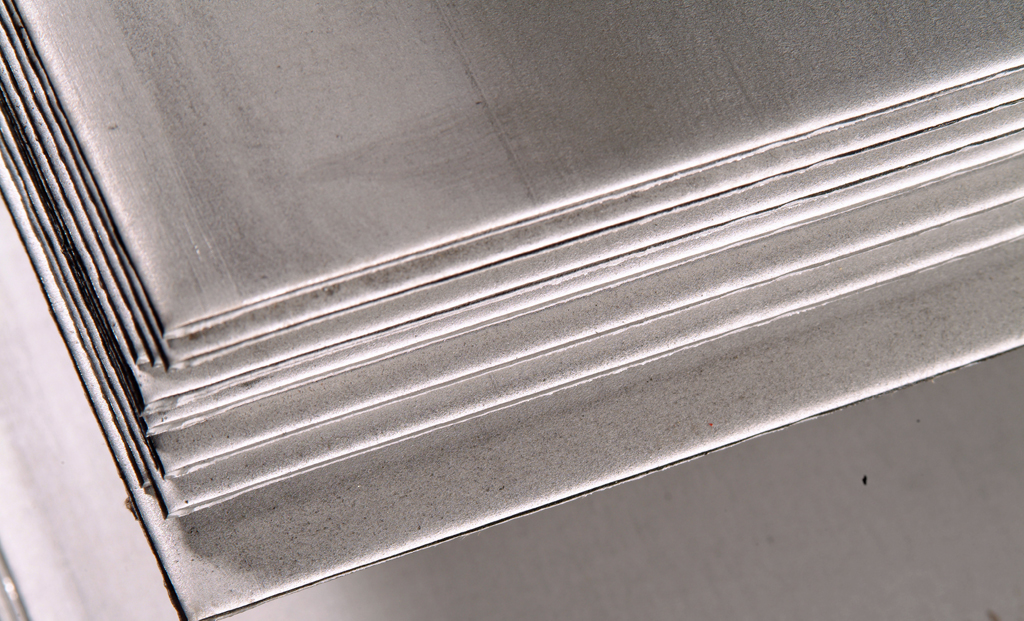
\includegraphics[width=0.75\textwidth]{Images/steel_plates_1.jpg}\\
				\vspace{0.5cm}
			    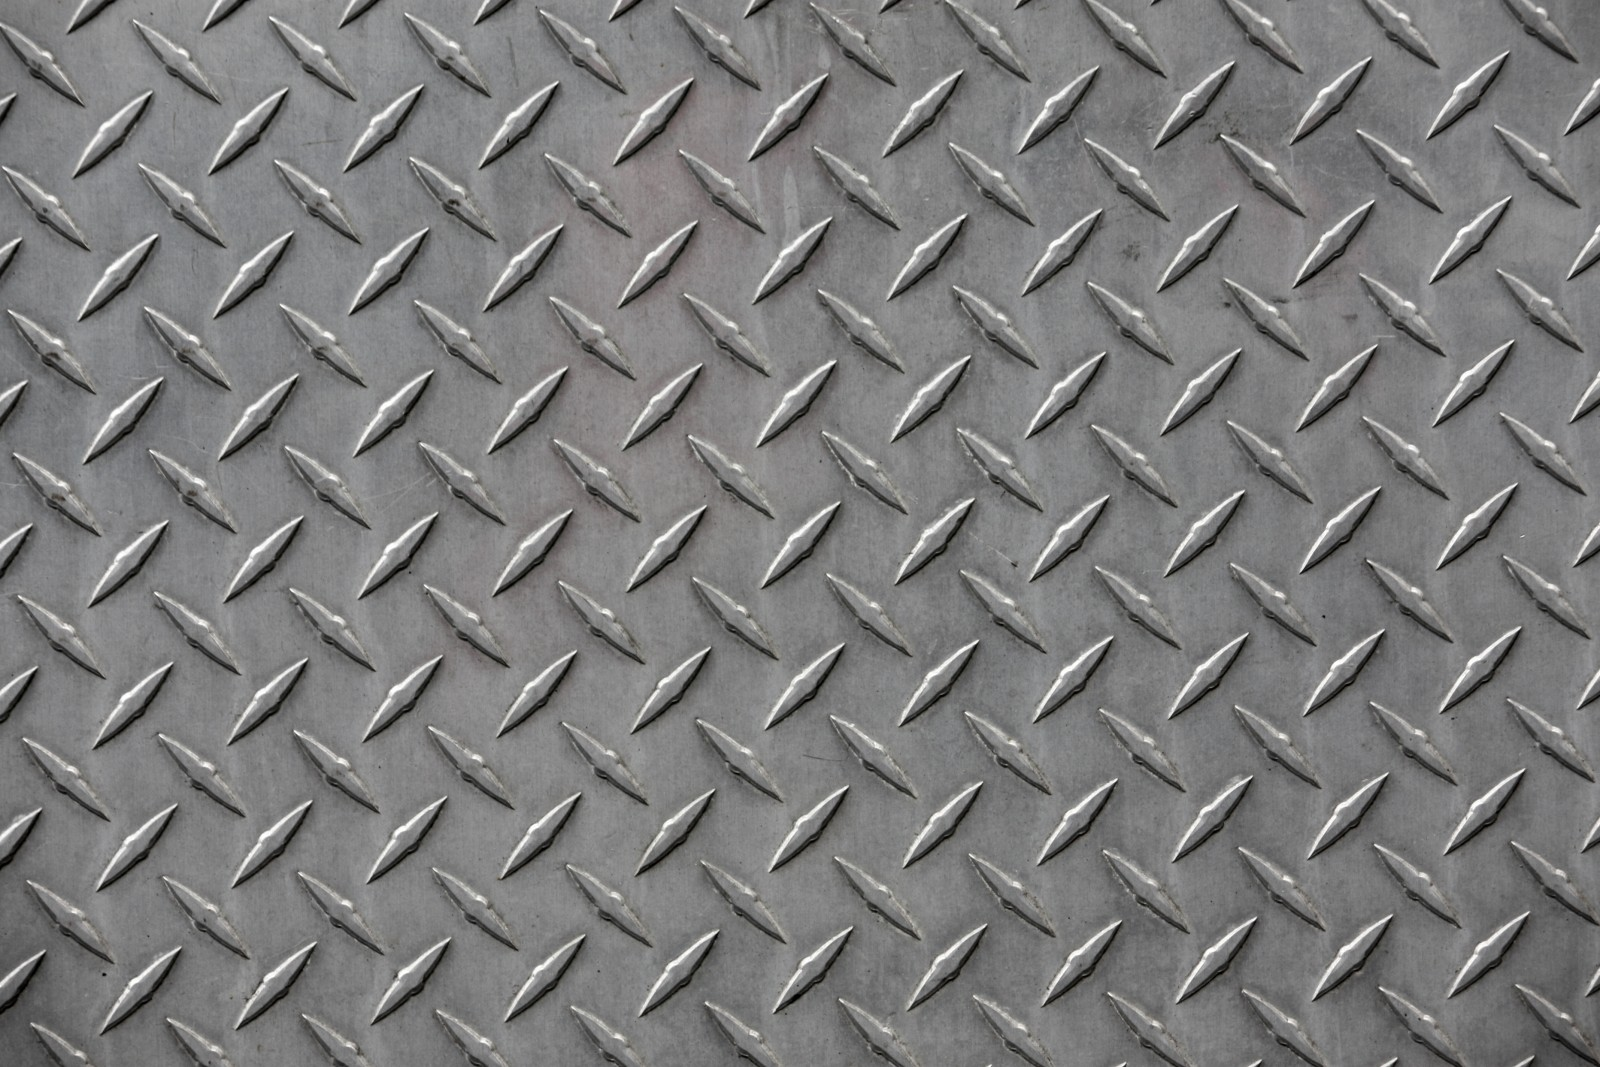
\includegraphics[width=0.75\textwidth]{Images/steel_plates_2.jpg}
			\end{figure}
		\end{column}
	\end{columns}
\end{frame}

\begin{frame}
	\frametitle{Preliminary analysis}
	\begin{figure}
		\centering
		\begin{subfigure}[b]{0.49\textwidth}
			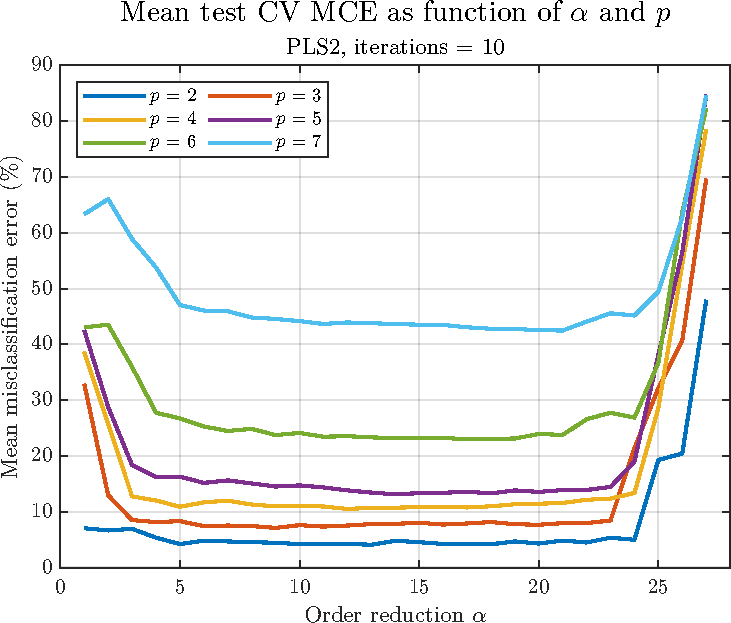
\includegraphics[width=\textwidth]{Images/trend_alpha_p_PLS2.pdf}
		\end{subfigure}
		\hfill
		\begin{subfigure}[b]{0.49\textwidth}
			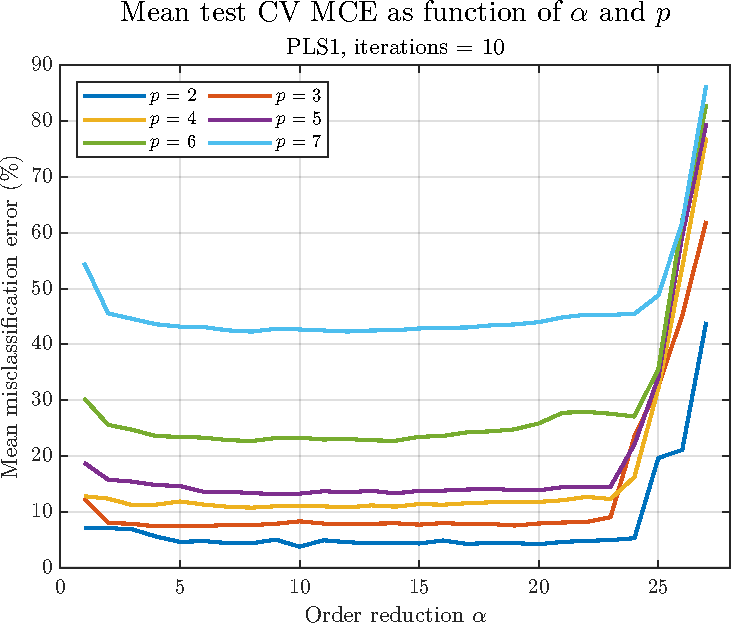
\includegraphics[width=\textwidth]{Images/trend_alpha_p_PLS1.pdf}
		\end{subfigure}
	\end{figure}
	As the number of fault classes \textit{p} taken into consideration increases, the mean test CV MCE also increases. Both algorithms show a similar behaviour in case of overfitting, while PLS1 underfits less than PLS2. 
\end{frame}

\begin{frame}
	\frametitle{Methodology}
	To reduce the dependency on a specific dataset randomization during the $10$-folds cross-validation, we decided to iterate this procedure $n$ times ($10$ in preliminary analysis). We used the CV technique to make inference on the model parameters, especially to choose the best model reduction $\alpha$.\\ As we can see from graphs in the previous frame, with $p = 5$ we obtain a model that is a good compromise between complexity and cross-validation performances, therefore we decided to make our in-depth analysis with this model.
\end{frame}

\begin{frame}
	\frametitle{In-depth analysis with $p = 5$}
	\begin{figure}
		\centering
		\begin{subfigure}[b]{0.49\textwidth}
			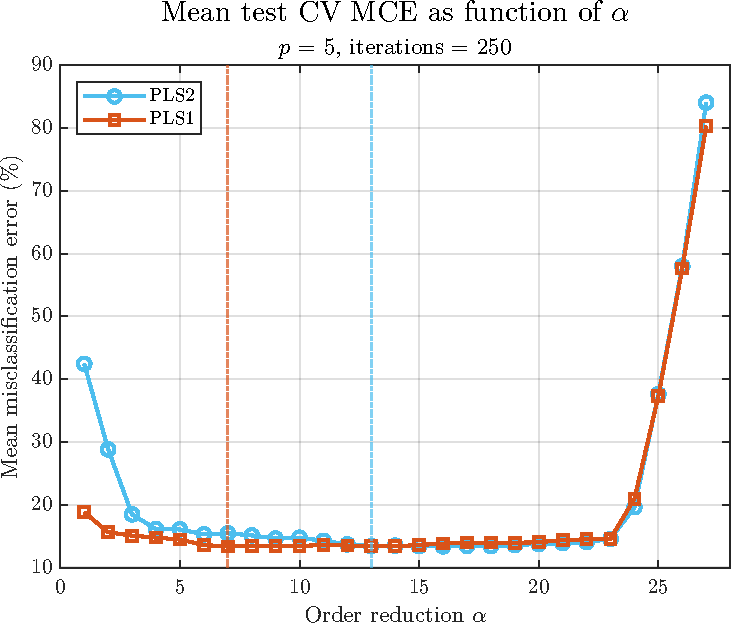
\includegraphics[width=\textwidth]{Images/trend_alpha_5.pdf}
		\end{subfigure}
		\hfill
		\begin{subfigure}[b]{0.49\textwidth}
			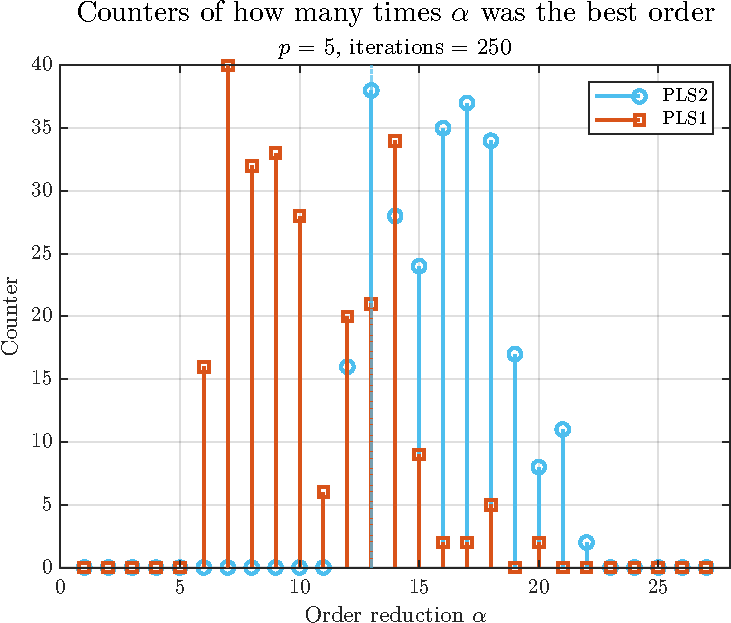
\includegraphics[width=\textwidth]{Images/counters_alpha_5.pdf}
		\end{subfigure}
	\end{figure}
	In the right figure we can note that PLS2 tends to advise more complex models than PLS1. This behaviour is confirmed by the left graph: PLS2 goes underfit faster than the other algorithm.
\end{frame}

\begin{frame}
	\begin{figure}
		\centering
		\begin{subfigure}[b]{0.60\textwidth}
			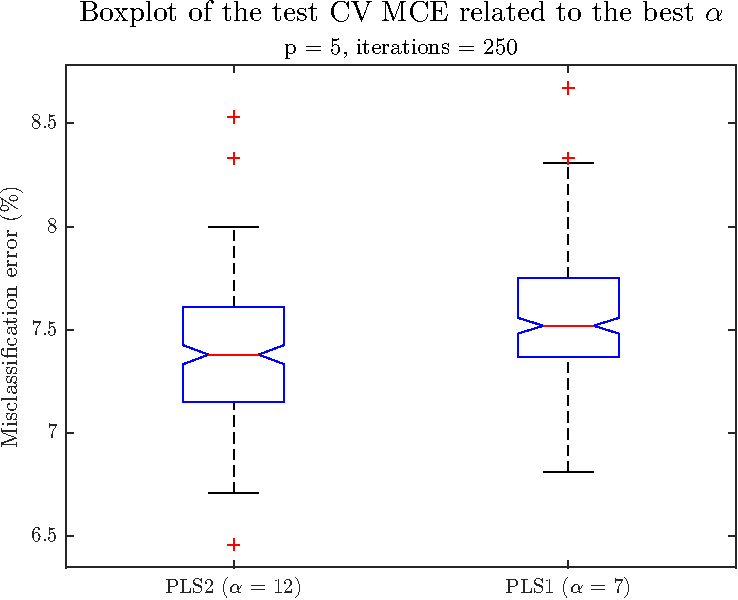
\includegraphics[width=\textwidth]{Images/box_alpha_5.pdf}
		\end{subfigure}
	\end{figure}
	Although PLS1 performs slightly better on average than PLS2, we decided to use the latter one for the following analyses because it is the model with the shortest estimation time.
\end{frame}

\begin{frame}
	\frametitle{Validation $70/30$ of the PLS2 model with $\alpha = 13$}
	\begin{figure}
		\begin{subfigure}[b]{0.49\textwidth}
			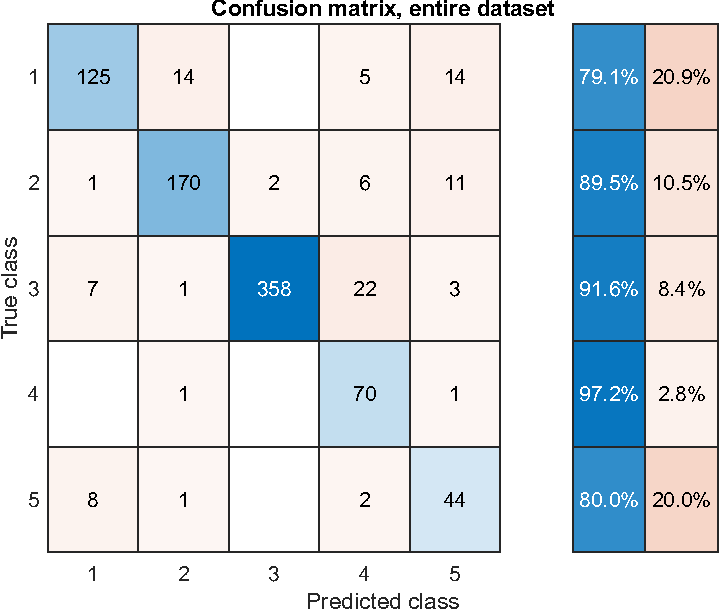
\includegraphics[width=\textwidth]{Images/confusion_all_5_PLS2.pdf}
		\end{subfigure}
		\hfill
		\begin{subfigure}[b]{0.49\textwidth}
			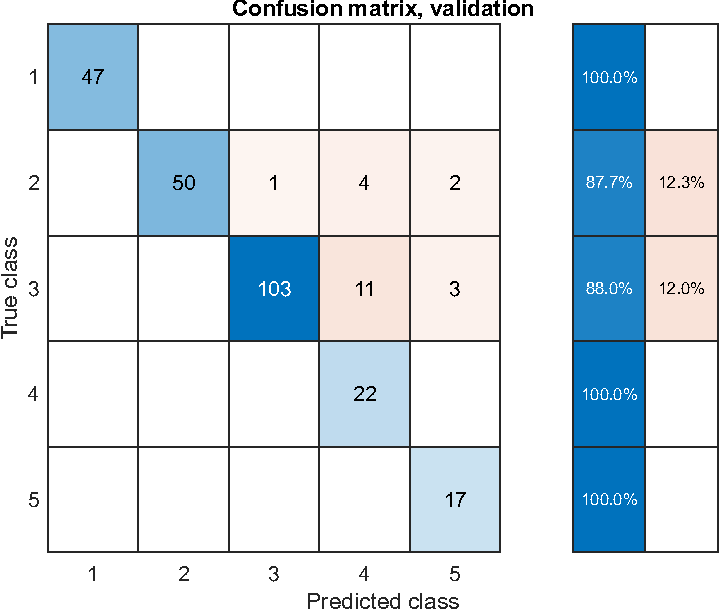
\includegraphics[width=\textwidth]{Images/confusion_val_5_PLS2.pdf}
		\end{subfigure}
	\end{figure}
	We can see that in validation there is a natural decrease in the predictive capabilities of the model. In particular, the fault classes on which PLS2 struggles the most are classes $1$ and $5$.
\end{frame}

\begin{frame}
	\frametitle{Score matrix $T$ with $\alpha = 1$, $2$ and $3$}
	\begin{figure}
		\begin{subfigure}[b]{0.70\textwidth}
			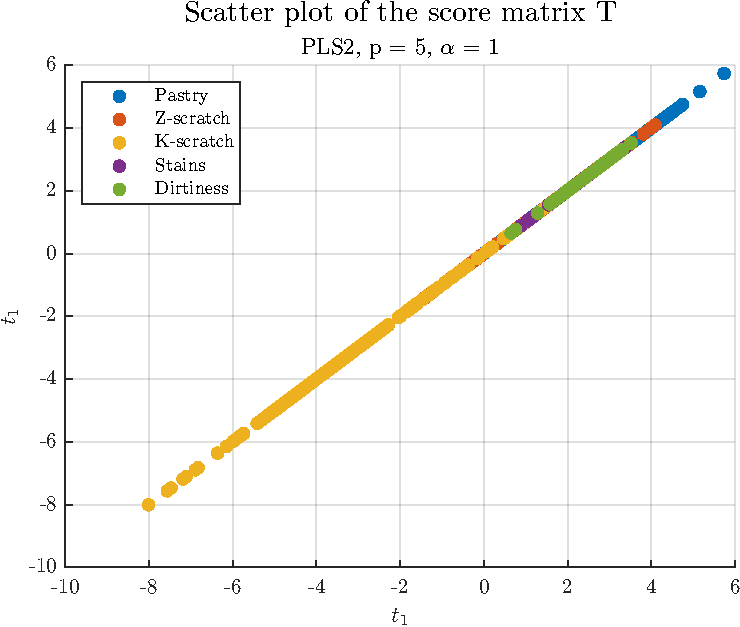
\includegraphics[width=\textwidth]{Images/scatter_T_a1_p5.pdf}
		\end{subfigure}
	\end{figure}
\end{frame}

\begin{frame}
	\begin{figure}
		\begin{subfigure}[b]{0.70\textwidth}
			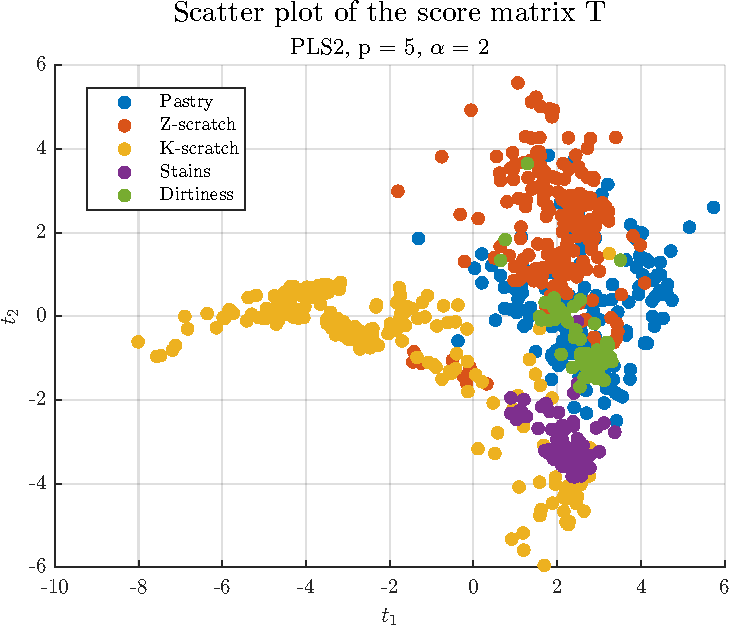
\includegraphics[width=\textwidth]{Images/scatter_T_a2_p5.pdf}
		\end{subfigure}
	\end{figure}
\end{frame}

\begin{frame}
	\begin{figure}
		\begin{subfigure}[b]{0.80\textwidth}
			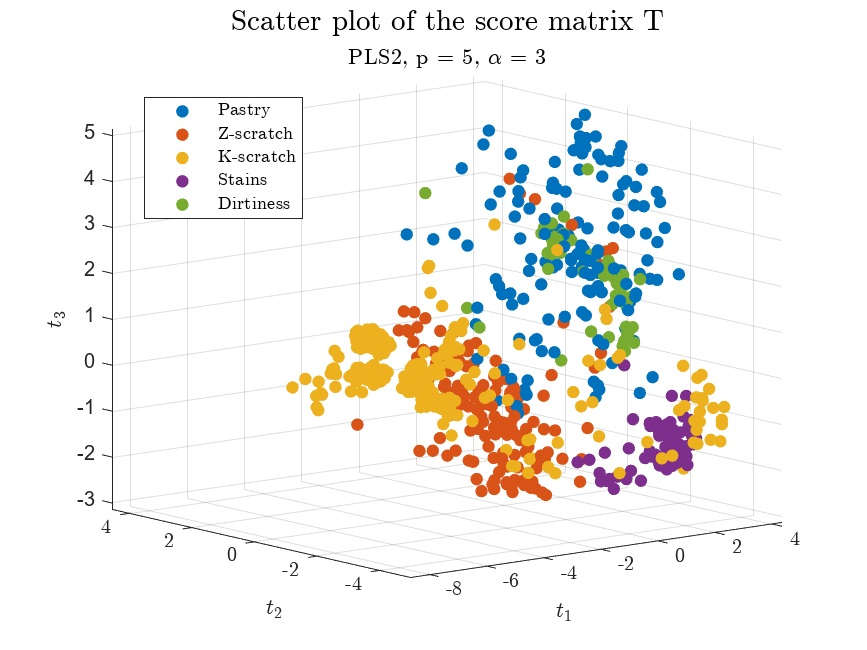
\includegraphics[width=\textwidth]{Images/scatter_T_a3_p5.pdf}
		\end{subfigure}
	\end{figure}
\end{frame}

\begin{frame}
	\begin{table}
		\centering
		\renewcommand\arraystretch{1.3}
		\begin{tabular}{c|c|c|c|c|c|c}
			\hline
			$\boldsymbol{\alpha}$ & \textbf{Pastry} & \textbf{Z-scratch} & \textbf{K-scratch} & \textbf{Stains} & \textbf{Dirtiness} & \textbf{Average}\\
			\hline
			\num{1} & $1.27\%$ & $100\%$ & $11.76\%$ & $100\%$ & $100\%$ & $42.15\%$ \\
			\num{2} & $77.85\%$ & $8.95\%$ & $12.53\%$ & $1.39\%$ & $100\%$ & $28.29\%$ \\
			\num{3} & $15.82\%$ & $10\%$ & $14.58\%$ & $1.39\%$ & $100\%$ & $18.13\%$ \\ 
			\hline
		\end{tabular}
	\end{table}
	As the order reduction $\alpha$ increases, the number of fault classes that are confused with the remaining ones decreases. In particular, we can note that the error rate related to the fault class Stains decreases substantially in the passage from $\alpha = 1$ to $\alpha = 2$; indeed, from $\mathbb{R}^2$ its subspace predominates over the subspaces of the other classes. Instead, the Dirtiness class continues to be hidden from the others for any order reduction. 
\end{frame}
	\section{Conclusion}

\begin{frame}
	TO DO
\end{frame}
	
\end{document}